\documentclass[a4paper,oneside,12pt]{report}
% Package yang diperlukan
\usepackage{fontspec}       % Font sistem untuk XeLaTeX/LuaLaTeX
\usepackage{setspace}       % Pengaturan jarak antarbaris
\usepackage{graphicx}      % Untuk memasukkan gambar
\usepackage{titling}       % Untuk kustomisasi halaman judul
\usepackage{geometry}      % Untuk mengatur margin halaman
\usepackage{listings}      % Untuk menampilkan blok kode
\usepackage{xcolor}        % Untuk menggunakan warna
\usepackage{float}         % Untuk kontrol penempatan float (seperti gambar)
\usepackage{hyperref}      % Untuk membuat hyperlink (URL, referensi)
\usepackage{indentfirst}   % Untuk memberi indentasi pada paragraf pertama setiap seksi
\usepackage{url}           % Untuk format URL
\usepackage{fancyhdr}      % Untuk kustomisasi header dan footer
\usepackage{tocloft}       % Untuk kustomisasi Daftar Isi
\usepackage{bookmark}      % Untuk manajemen bookmark PDF yang lebih baik

% Font dan spasi standar laporan praktikum
\setmainfont{TeX Gyre Termes}
\onehalfspacing

%======================================================================
% PENGATURAN GEOMETRI HALAMAN
%======================================================================
\geometry{left=3cm, right=2.5cm, top=2cm, bottom=2.5cm}
\sloppy

%======================================================================
% PENGATURAN WARNA UNTUK BLOK KODE
%======================================================================
\definecolor{codegreen}{rgb}{0,0.6,0}
\definecolor{codegray}{rgb}{0.5,0.5,0.5}
\definecolor{codepurple}{rgb}{0.58,0,0.82}
\definecolor{backcolour}{rgb}{0.95,0.95,0.92}
\definecolor{darkblue}{rgb}{0,0,0.6}

%======================================================================
% PENGATURAN BLOK KODE (LISTINGS)
%======================================================================
\lstdefinestyle{commonstyle}{
    backgroundcolor=\color{backcolour},
    breakatwhitespace=false,
    breaklines=true,
    captionpos=b,
    keepspaces=true,
    numbers=left,
    numbersep=5pt,
    showspaces=false,
    showstringspaces=false,
    showtabs=false,
    tabsize=2,
    frame=single,
    basicstyle=\ttfamily\footnotesize,
    numberstyle=\tiny\color{codegray},
    columns=flexible,
    postbreak=\mbox{\textcolor{red}{$\hookrightarrow$}\space},
    breakindent=0pt,
    breakautoindent=false
}

%======================================================================
% PENGATURAN LAIN-LAIN
%======================================================================
\newcommand{\customfbox}[1]{%
  \setlength{\fboxsep}{0pt}%
  \setlength{\fboxrule}{0.5pt}%
  \fcolorbox{black}{white}{#1}%
}
\renewcommand{\figurename}{Gambar}
\renewcommand{\thefigure}{\arabic{figure}}
\hypersetup{
    colorlinks=true,
    linkcolor=black,
    filecolor=black,
    urlcolor=black,
    citecolor=black,
    pdftitle={Laporan Praktikum PPG Pertemuan 2},
    pdfpagemode=UseOutlines,
    breaklinks=true
}
\pagestyle{fancy}
\fancyhf{}
\fancyfoot[C]{\thepage}
\renewcommand{\headrulewidth}{0pt}
\fancypagestyle{plain}{
    \fancyhf{}
    \fancyfoot[C]{\thepage}
    \renewcommand{\headrulewidth}{0pt}
}
\renewcommand{\contentsname}{Daftar Isi}
\renewcommand{\bibname}{Daftar Pustaka}
\renewcommand{\thechapter}{}
\renewcommand{\chaptername}{}
\renewcommand{\thesection}{\arabic{chapter}.\arabic{section}}
\renewcommand{\thesubsection}{\thesection.\arabic{subsection}}
\setcounter{secnumdepth}{3}
\setcounter{tocdepth}{3}
\renewcommand{\cftchapdotsep}{\cftdotsep}
\renewcommand{\cftchapleader}{\cftdotfill{\cftchapdotsep}}
\setlength{\cftchapindent}{0em}
\setlength{\cftsecindent}{2em}
\setlength{\cftsubsecindent}{4em}
\setlength{\cftchapnumwidth}{0em}
\setlength{\cftsecnumwidth}{2.5em}
\setlength{\cftsubsecnumwidth}{3.2em}
\renewcommand{\cftchappresnum}{}
\renewcommand{\cftchapaftersnum}{}
\newcommand{\tocboldsection}[1]{%
  \protect\renewcommand{\protect\cftchapfont}{\protect\bfseries}%
  #1%
  \protect\renewcommand{\protect\cftchapfont}{}%
}

%======================================================================
% AWAL DOKUMEN
%======================================================================
\begin{document}

% Halaman Judul
\newgeometry{left=3cm, right=2.5cm, top=2.5cm, bottom=3cm}
\begin{titlingpage}
\begin{spacing}{1}
\begin{center}
\vspace*{0.2cm}
{\large \textbf{\MakeUppercase{Laporan Praktikum}}} \\[0.4cm]
{\large \textbf{\MakeUppercase{PRAKTIKUM PENGEMBANGAN GAME}}} \\[0.4cm]
{\large \textbf{\MakeUppercase{Pertemuan 2}}} \\[0.4cm]
{\large \textbf{\MakeUppercase{NAVIGATE UNREAL ENGINE 5.8}}} \\[1.5cm]


\includegraphics[height=7cm]{images/UGM.png} \\[0.7cm]

{\normalsize \textbf{Disusun oleh:}} \\[0.4cm]
\begin{tabular}{@{}l l @{}}
  \textbf{Nama}           & : Hafidz Rizqullah Prasetya \\
  \textbf{NIM}            & : 24/535493/SV/24243 \\
  \textbf{NIU}            & : 535493 \\
  \textbf{Kelas}          & : PL5A1 \\
  \textbf{Dosen Pengampu} & : Yusron Fuadi, S.Sn., M.Sn. \\
  \textbf{Asisten}        & : Ezra Bariq Rizqullah / Ikhwan Hanif Firdaus \\
\end{tabular} \\[1.2cm]

{\normalsize \textbf{PROGRAM STUDI D-IV}} \\[0.2cm]
{\normalsize \textbf{TEKNOLOGI REKAYASA PERANGKAT LUNAK}} \\[0.2cm]
{\normalsize \textbf{DEPARTEMEN TEKNIK ELEKTRO DAN INFORMATIKA}} \\[0.2cm]
{\normalsize \textbf{SEKOLAH VOKASI}} \\[0.2cm]
{\normalsize \textbf{UNIVERSITAS GADJAH MADA}} \\[0.2cm]
{\normalsize \textbf{YOGYAKARTA}} \\[0.2cm]
{\normalsize \textbf{2026}} \\[1.2cm]
\end{center}
\end{spacing}
\end{titlingpage}
\restoregeometry

\thispagestyle{empty}
\clearpage
\stepcounter{page}
\thispagestyle{empty}

% --- Daftar Isi ---
\addcontentsline{toc}{chapter}{Daftar Isi}
\tableofcontents
\clearpage

% Mengatur penomoran halaman menjadi arab dan mulai dari 3
\pagenumbering{arabic}
\setcounter{page}{3}

\chapter[Tujuan Praktikum]{Tujuan Praktikum}
\begin{enumerate}
   \item Mahasiswa mampu memahami konsep dasar Unreal Engine 5.8 sebagai engine real-time lintas platform dari Epic Games beserta model lisensinya \cite{epic-unreal}.
   \item Mahasiswa mampu mengoperasikan Epic Games Launcher untuk manajemen instalasi engine dan project, termasuk penanganan warning file \texttt{.uproject} dan akses Library \cite{modul2}.
   \item Mahasiswa mampu menavigasi antarmuka editor Unreal Engine 5.8 yang meliputi Outliner, Details, Viewport, Content Drawer, dan Top Bar, serta memahami fungsi navigasi dasar seperti PLAY, STOP, dan transformasi objek \cite{modul2}.
   \item Mahasiswa mampu melakukan manipulasi objek dan material, pengaturan collision dan physics, pencahayaan Point Light, sistem particle Niagara, Sequencer, serta logika Blueprint dan penyimpanan project sesuai alur praktikum \cite{epic-variants}.
\end{enumerate}
\clearpage

\chapter{Dasar Teori}

\section{Unreal Engine dan Ekosistem Epic Games}
Unreal Engine dikembangkan oleh Epic Games, perusahaan yang juga dikenal lewat Fortnite. Pemakaiannya tidak berhenti di game. Engine ini juga dipakai di industri film, arsitektur, otomotif, dan simulasi, pokoknya bidang yang butuh visual bagus dengan performa real-time \cite{modul2,epic-unreal}. Dari modul saya paham bahwa fitur yang tersedia di dalamnya setara dengan yang dipakai studio AAA, jadi engine ini sanggup dipakai untuk pipeline agile maupun produksi kompleks yang melibatkan banyak disiplin.

Soal lisensi, Unreal Engine gratis dipakai selama tahap pengembangan. Royalti 5\% baru muncul kalau game-nya dirilis secara komersial dan pendapatan kotornya sudah lewat 1.000.000 USD \cite{modul2}. Buat mahasiswa seperti saya, skema ini jelas menguntungkan karena bisa belajar penuh tanpa keluar biaya di awal.

\section{One Engine for All Platform}
Unreal Engine bisa melakukan deploy build ke banyak platform sekaligus, yaitu PC (Windows, Mac, Linux), console (PS5, Xbox), dan mobile (iOS, Android) \cite{modul2,epic-variants}. Menurut saya kemampuan lintas platform ini penting, karena logika game tidak perlu ditulis ulang dari nol untuk tiap platform.

Contoh paling ekstrem yang disebutkan di modul adalah Kuro Games. Mereka merilis game open-world masif Wuthering Waves memakai versi modifikasi Unreal Engine, dan berhasil melakukan update live serentak di PC, console, bahkan perangkat mobile low-end pada hari yang sama \cite{kurogames,wuthering-cover}. Dari studi kasus itu kelihatan bahwa Unreal cukup fleksibel untuk menangani optimasi lintas perangkat yang jarak spesifikasinya jauh.

\section{Epic Games Launcher sebagai Hub Manajemen}
Pintu masuk ke Unreal Engine adalah Epic Games Launcher. Dari launcher ini saya buka menu Unreal Engine $>$ Library untuk melihat versi engine yang terpasang dan daftar project di segmen ``MY PROJECTS'' \cite{modul2}.

Launcher juga bisa mendeteksi file project berekstensi \texttt{.uproject} yang belum terdaftar. Kalau warning seperti itu muncul, instruksi modulnya sederhana: klik ``FIX NOW'' supaya project dikenali lagi oleh launcher \cite{modul2}. Setelah beres, engine dibuka dengan klik \textbf{Launch} pada versi 5.8.1.

\section{Manajemen Project dan Template}
Begitu engine jalan, Home Window muncul dengan akses terpusat ke dokumentasi, sample projects, dan tutorial. Untuk bikin project baru, saya klik \textbf{New Project} dan masuk ke window New Projects \cite{modul2,epic-variants}.

Di window inilah template dikonfigurasi. Sesuai instruksi praktikum pertemuan 2, saya memilih \textbf{GAMES $>$ Intro To Unreal} lalu mengubah nama project dengan format \textbf{NAMA\_NIU\_Intro}, contohnya \texttt{HAFIDZ\_535493\_Intro} \cite{modul2}. Format penamaan ini wajib diikuti supaya tugas gampang diidentifikasi. Catatan kecil: pada pertemuan 3 templatenya diganti ke Third Person karena ada bug rigging di IntroToUnreal, tapi untuk pertemuan 2 tetap pakai Intro To Unreal.

Setelah project dibuat, layar loading muncul. Modul menyelipkan satu ``Useless Fact'' di sini: gambar loading itu bisa diganti dengan gambar custom yang berbeda untuk tiap project \cite{modul2}.

\section{Antarmuka Utama Editor Unreal Engine 5.8}
\subsection{Outliner, Details, dan Viewport}
Setelah loading selesai, editor terbuka dengan sambutan ``Welcome To The Editor!'' \cite{modul2}. Ada tiga panel inti yang paling sering dipakai:

\begin{itemize}
    \item \textbf{Outliner} berisi daftar semua objek atau actor yang ada dalam level, mulai dari mesh, light, camera, sampai Player Start. Panel ini memudahkan seleksi dan pencarian objek tanpa harus mencarinya satu per satu di Viewport \cite{modul2}.
    \item \textbf{Details} menampilkan properties dari objek yang sedang dipilih. Misalnya saat saya klik sebuah mesh, yang muncul adalah transform, material, collision, physics, dan lighting objek itu \cite{modul2}.
    \item \textbf{Viewport} adalah area kerja utama tempat scene terlihat secara visual. Navigasi kamera dan penempatan objek semuanya dilakukan di sini \cite{modul2}.
\end{itemize}

\subsection{Top Bar dan Content Drawer}
Top Bar memuat fungsi-fungsi yang sering dipakai: \textbf{Save Changes on Current Level}, \textbf{Switches editor workflow modes} (Landscape, Foliage, Mesh Paint, Modeling, Animation editing), \textbf{Add Objects}, \textbf{Blueprints Menu}, \textbf{Cinematics/Sequencer}, dan tombol \textbf{PLAY} \cite{modul2}. Sementara itu Content Drawer (Content Browser) bisa dibuka cepat dengan \texttt{CTRL + SPACE} dan berisi daftar aset project seperti mesh, material, texture, blueprint, dan map \cite{modul2}.

Untuk menjalankan simulasi, tombol Play dipakai untuk memulai, Escape untuk berhenti, dan SHIFT+F1 dipakai kalau kursor mouse mau dikeluarkan dari Viewport tanpa keluar dari mode Play \cite{modul2}.

\section{Transformasi, Grid, dan Manajemen Objek}
Transformasi objek mencakup Move/Translate, Rotate, dan Scale. Ketiganya dioperasikan lewat gizmo berbentuk panah, lingkaran, dan kotak yang muncul di Viewport \cite{modul2}. Grid membantu penempatan presisi dan bisa diaktifkan atau dimatikan sesuai kebutuhan. Untuk manajemen objek, penambahan dilakukan lewat menu Add Objects, sedangkan objek yang sulit diklik langsung di Viewport bisa dihapus lewat Outliner dengan cara diseleksi berdasarkan nama lalu delete \cite{modul2}.

Collision mengatur bagaimana objek berinteraksi secara fisik dengan objek lain, misalnya apakah objek menghalangi pergerakan atau bentuk collision-nya sederhana atau kompleks. Pengaturan ini ada di panel Details saat objek dipilih \cite{modul2}.

\section{Material, Hot-Swap, Particle, dan Physics}
Material menentukan tampilan permukaan objek lewat properti seperti Color, Metallic, dan Roughness. Penggantian material bisa dilakukan cepat lewat fitur Hot-Swap Material Slot di Details, tanpa perlu membuat ulang objek atau material dari awal \cite{modul2}.

Untuk efek visual, Unreal memakai Niagara Editor sebagai tempat mengatur particle system seperti api, asap, dan ledakan \cite{modul2}. Property physics yang mengatur gravitasi dan respons tabrakan juga diubah lewat Details. Menambahkan cahaya dilakukan dengan shortcut \texttt{L + Left Click} untuk Point Light, yaitu sumber cahaya yang memancar ke segala arah dari satu titik, mirip bola lampu \cite{modul2}.

\section{Sequencer, Blueprint Logic, dan Penyimpanan}
Sequencer adalah fitur untuk membuat cinematics dan cutscene. Masuknya lewat Outliner, dengan \textbf{Right Click $>$ Edit} pada objek terkait \cite{modul2}. Sementara itu logika objek diatur lewat Blueprint, sistem visual scripting Unreal. Lewat Blueprint, perilaku objek bisa ditentukan, misalnya apa yang terjadi ketika objek disentuh atau ditabrak \cite{modul2}.

Sebagai langkah penutup, semua perubahan disimpan lewat \textbf{Save Changes on Current Level} atau shortcut \texttt{CTRL + S} supaya progress tidak hilang \cite{modul2}.

\clearpage

\chapter[\tocboldsection{Hasil dan Pembahasan}]{Hasil dan Pembahasan}

Bab ini berisi dokumentasi praktikum Navigate Unreal Engine 5.8 sesuai Modul Pertemuan 2. Semua langkah saya kerjakan di Unreal Engine 5.8.1 lewat Epic Games Launcher, dan tiap langkah saya dokumentasikan dengan screenshot berikut keterangan singkatnya. Project yang saya buat bernama \texttt{HAFIDZ\_535493\_Intro} sesuai format yang diminta modul.

Satu hal yang perlu dicatat: template Intro To Unreal ternyata bukan level kosong, melainkan tutorial interaktif 16 stasiun. Jadi alur praktikumnya banyak berjalan mengikuti stasiun-stasiun tutorial tersebut sambil mencoba langsung fitur yang dijelaskan di tiap dindingnya.

\section{Dokumentasi Praktikum}

\subsection{Persiapan Awal: Epic Games Launcher dan Pembuatan Project}

\begin{enumerate}
    \item \textbf{Membuka Epic Games Launcher dan akses Unreal Engine $>$ Library.} Saya membuka Epic Games Launcher lalu masuk ke menu Unreal Engine $>$ Library untuk melihat engine yang sudah terpasang.

    \item \textbf{Menangani warning file .uproject.} Modul menginstruksikan klik \textbf{FIX NOW} kalau launcher mendeteksi file \texttt{.uproject} yang tidak terdaftar. Pada percobaan saya warning ini tidak muncul, jadi langkahnya hanya saya siapkan sebagai antisipasi.

    \item \textbf{Launch Unreal Engine 5.8.1.} Saya klik \textbf{Launch} pada engine versi 5.8.1. Project yang pernah dibuat sebelumnya muncul di segmen ``MY PROJECTS''.

    \item \textbf{Home Window dan klik New Project.} Setelah engine terbuka, Home Window muncul dengan akses ke dokumentasi, sample projects, dan tutorial. Dari sini saya klik \textbf{New Project}.

    \item \textbf{Window New Projects: pilih GAMES $>$ Intro To Unreal.} Saya memilih template \textbf{GAMES $>$ Intro To Unreal} dan mengganti Project Name menjadi \texttt{HAFIDZ\_535493\_Intro} sesuai format NAMA\_NIU\_Intro.

    \item \textbf{Menunggu loading project.} Setelah project dibuat, saya menunggu proses loading sampai selesai. Seperti ``Useless Fact'' di modul, gambar loading ini sebenarnya bisa diganti custom per project.
\end{enumerate}

\subsection{Eksplorasi Antarmuka Editor}

\begin{enumerate}
    \item \textbf{Masuk editor Lvl\_IntroRoom.} Project terbuka langsung pada level \texttt{Lvl\_IntroRoom} dengan overlay ``Welcome to Unreal Engine 5!'' yang memandu navigasi dasar. Di Outliner terlihat level ini berisi 407 actors dengan folder seperti Bridge, Lighting, dan Room\_Animation. Saat saya klik objek \texttt{SM\_Cube12}, panel Details menampilkan Transform (Location 150, 100, 750; Scale 12, 3, 0.505), Static Mesh \texttt{SM\_Cube}, dan material \texttt{MI\_Intro\_Colorway}.

\begin{figure}[H]
    \centering
    \customfbox{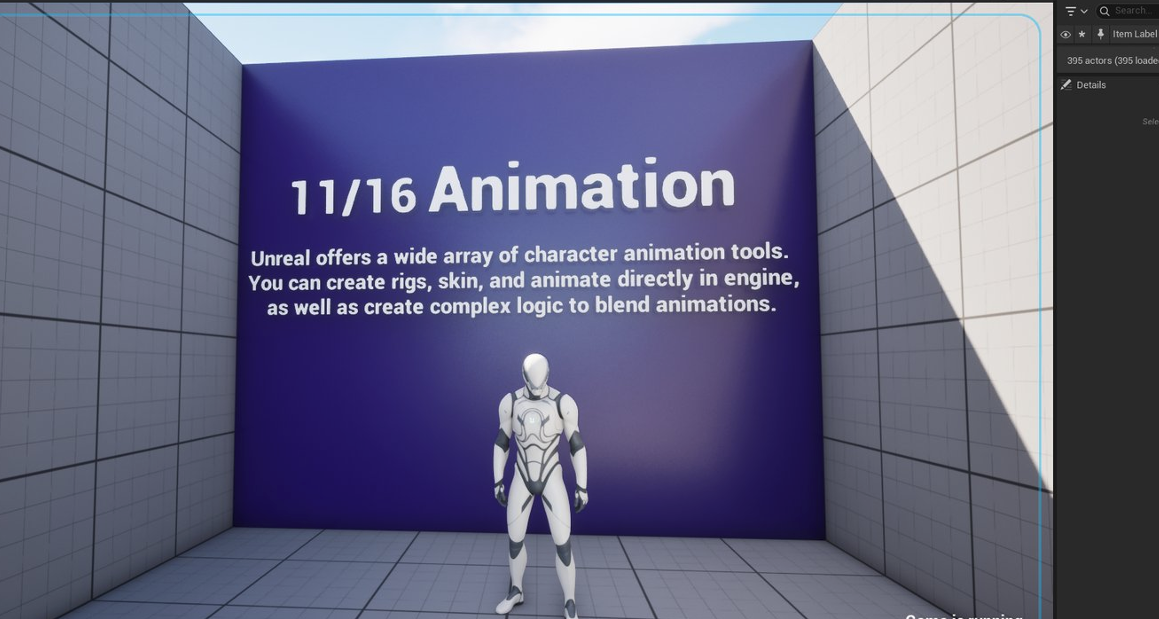
\includegraphics[width=0.85\textwidth]{images/ss-22-viewport-interior.png}}
    \caption{Tampilan awal editor Lvl\_IntroRoom dengan overlay Welcome to Unreal Engine 5.}
    \label{fig:ss-welcome}
\end{figure}

\begin{figure}[H]
    \centering
    \customfbox{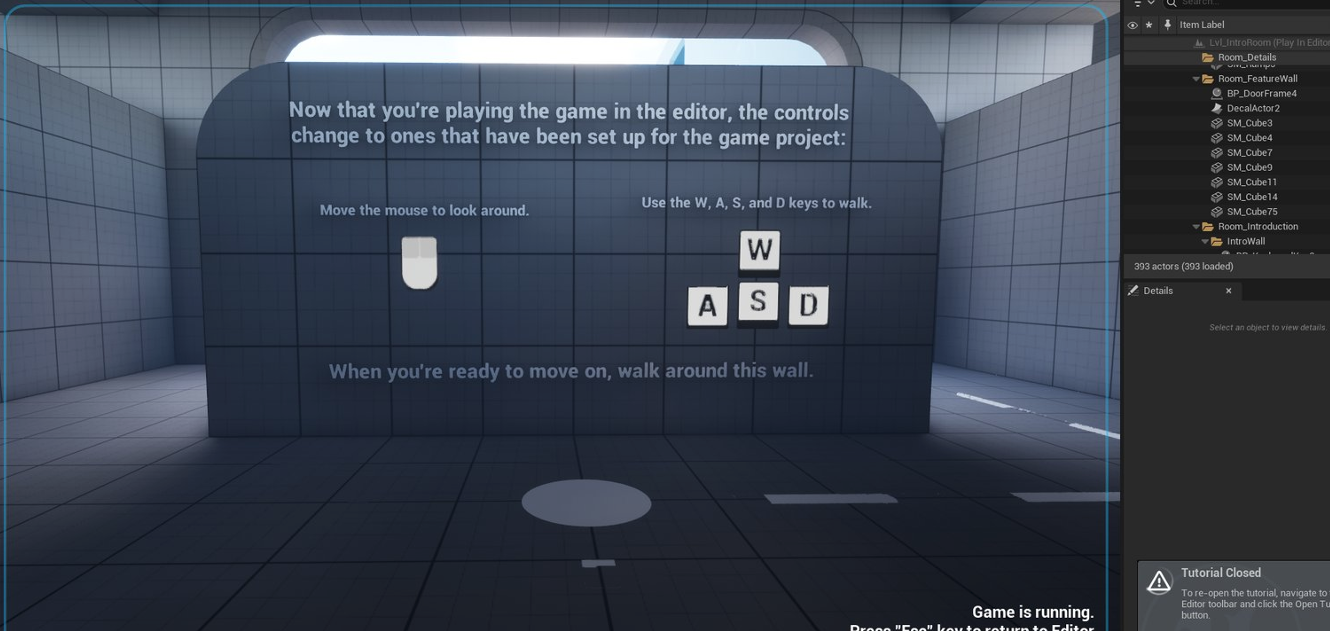
\includegraphics[width=0.55\textwidth]{images/ss-07-play-stop.png}}
    \caption{Outliner Lvl\_IntroRoom berisi 407 actors dengan folder Bridge, Lighting, dan Room\_Animation.}
    \label{fig:ss-outliner}
\end{figure}

\begin{figure}[H]
    \centering
    \customfbox{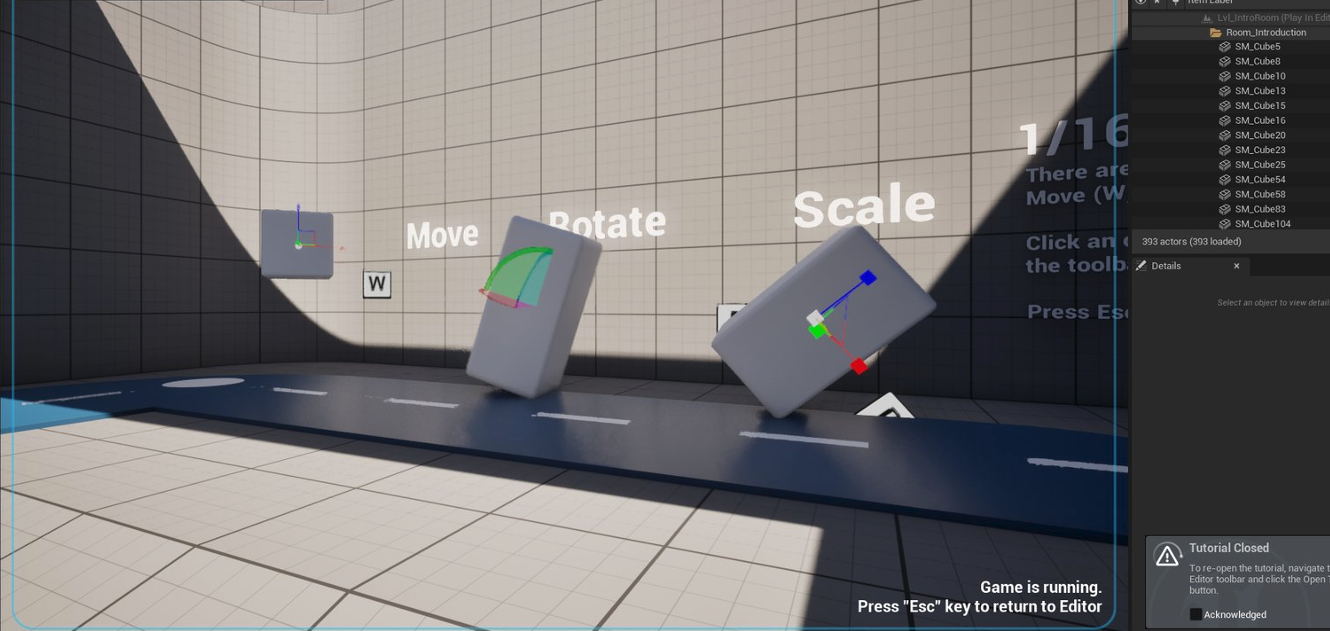
\includegraphics[width=0.65\textwidth]{images/ss-08-transform.png}}
    \caption{Panel Details objek SM\_Cube12: Transform, Static Mesh SM\_Cube, dan material MI\_Intro\_Colorway.}
    \label{fig:ss-details}
\end{figure}

    \item \textbf{Navigasi Viewport dengan fly mode.} Saya mencoba navigasi kamera di Viewport memakai kombinasi klik kanan mouse (RMB) plus tombol WASD untuk bergerak dan QE untuk naik-turun. Dari area luar bangunan, terlihat ramp menuju dinding stasiun 8/16 Atmosphere dengan langit biru berawan di atasnya. Di sinilah perbedaan kecepatan gerak kamera mulai terasa saat scroll mouse diputar.

\begin{figure}[H]
    \centering
    \customfbox{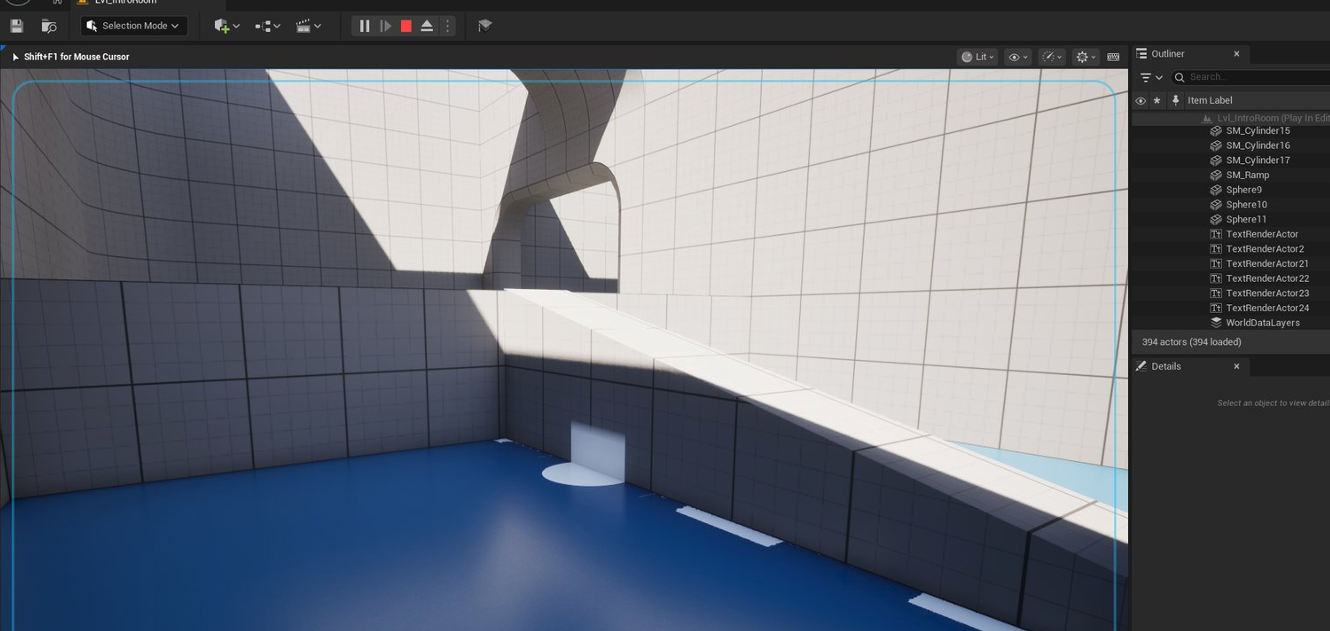
\includegraphics[width=0.9\textwidth]{images/ss-26-viewport-ramp.png}}
    \caption{Navigasi Viewport menuju stasiun 8/16 Atmosphere dengan langit biru dan ramp akses ke bangunan utama.}
    \label{fig:ss-viewport}
\end{figure}

    \item \textbf{Menguji PLAY dan kontrol di dalam game.} Saya klik tombol Play hijau di Top Bar. Mode Play langsung aktif dan kontrol berubah mengikuti setup project: mouse untuk melihat sekitar, WASD untuk berjalan. Di bagian bawah layar muncul tulisan ``Game is running. Press Esc key to return to Editor'', dan notifikasi ``Tutorial Closed'' muncul di kanan bawah. Setelah selesai mencoba, saya menekan Escape untuk berhenti. SHIFT+F1 saya pakai saat butuh mengeluarkan kursor tanpa keluar dari mode Play.

\begin{figure}[H]
    \centering
    \customfbox{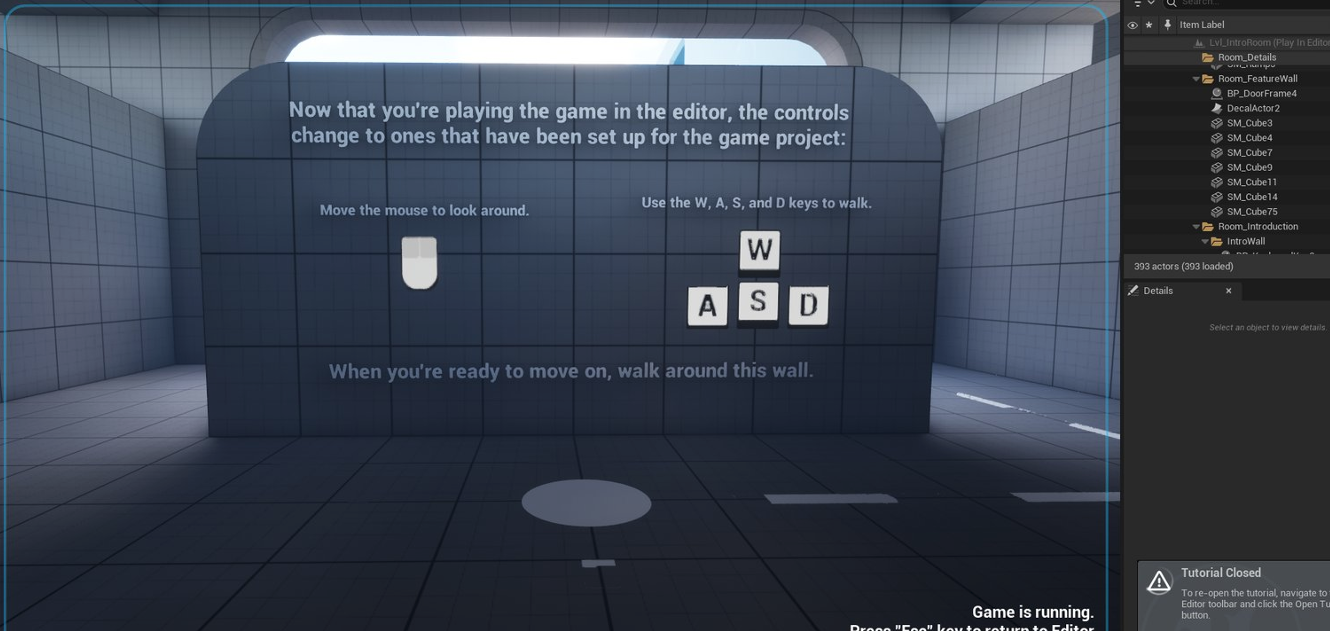
\includegraphics[width=0.9\textwidth]{images/ss-07-play-stop.png}}
    \caption{Mode Play aktif di Lvl\_IntroRoom: kontrol berubah ke mouse + WASD, dengan status ``Game is running'' di bagian bawah viewport.}
    \label{fig:ss-play}
\end{figure}
\end{enumerate}

\subsection{Manipulasi Objek, Material, dan Aset}

\begin{enumerate}
    \item \textbf{Transform Object: Move, Rotate, Scale.} Di stasiun 1/16 Moving Objects, saya mencoba tiga mode transformasi. Objek kubus di stasiun ini menampilkan gizmo sesuai mode yang dipilih: panah untuk Move, busur lingkaran untuk Rotate, dan kotak untuk Scale. Teks di dinding menandai ketiga mode itu dengan label ``Move'', ``Rotate'', dan ``Scale'' besar.

\begin{figure}[H]
    \centering
    \customfbox{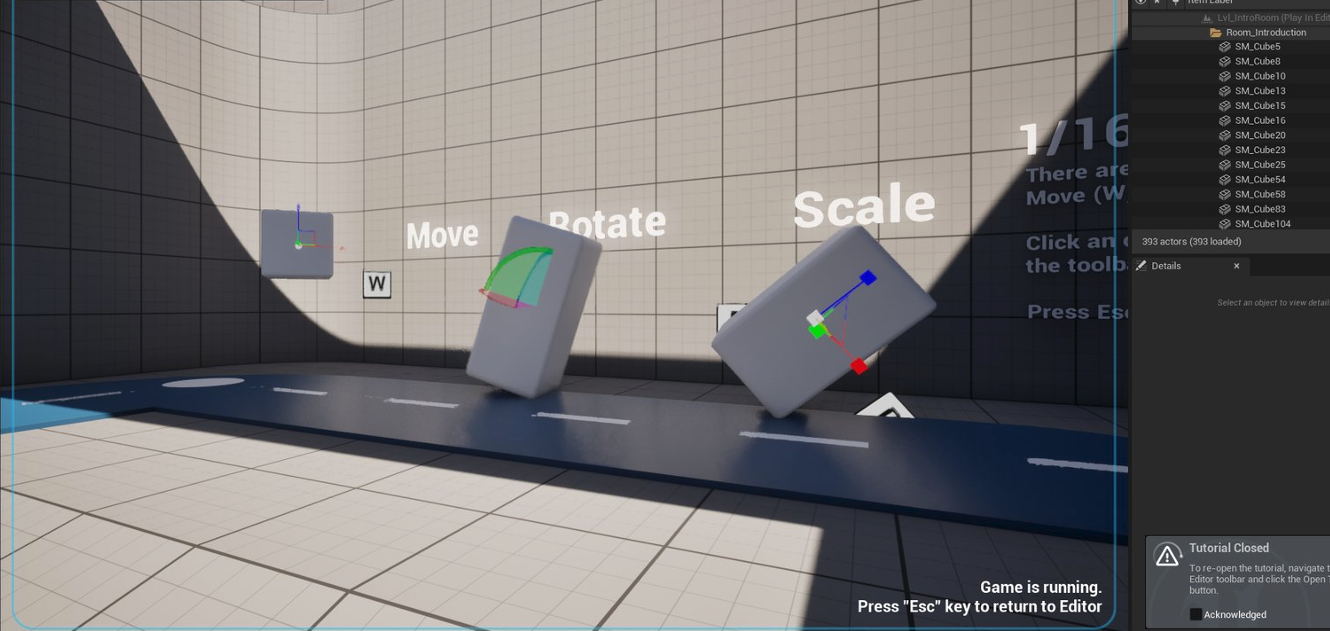
\includegraphics[width=0.9\textwidth]{images/ss-08-transform.png}}
    \caption{Stasiun 1/16 Moving Objects: percobaan gizmo Move, Rotate, dan Scale pada kubus.}
    \label{fig:ss-transform}
\end{figure}

    \item \textbf{Enable/Disable Grid.} Saya mengaktifkan dan mematikan grid lewat ikon grid di toolbar atas Viewport, lengkap dengan pengaturan ukuran snap-nya. Saat grid aktif, garis bantu muncul di lantai viewport dan objek lebih gampang disejajarkan; saat dimatikan, tampilan viewport jadi lebih bersih.

\begin{figure}[H]
    \centering
    \customfbox{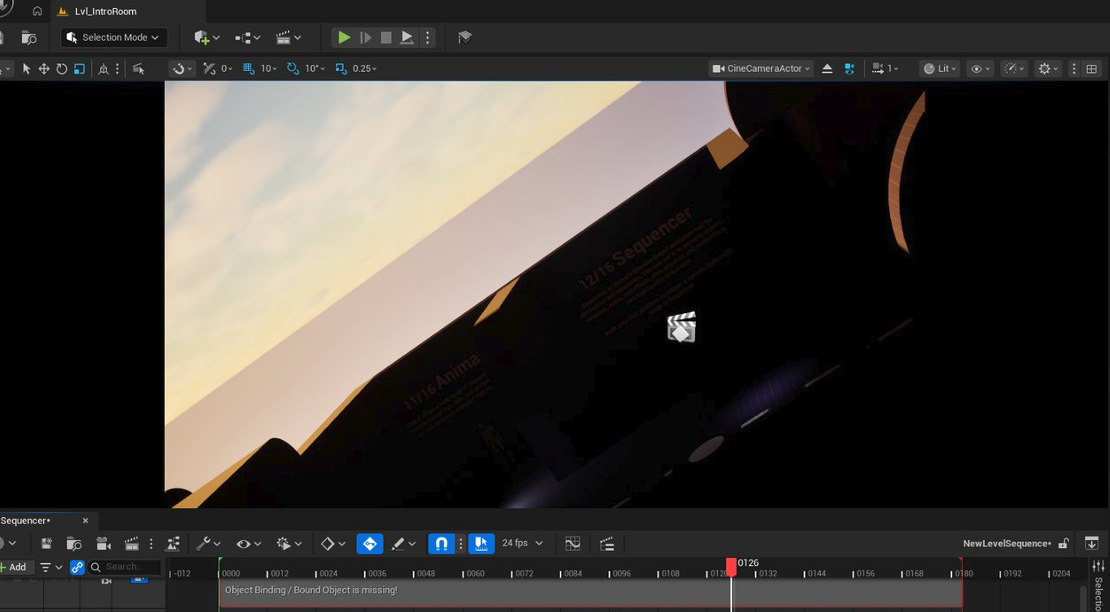
\includegraphics[width=0.9\textwidth]{images/ss-19-sequencer.png}}
    \caption{Pengaturan grid pada toolbar Viewport untuk penempatan objek yang presisi.}
    \label{fig:ss-grid}
\end{figure}

    \item \textbf{Menambahkan objek ke level.} Saya menekan ikon kubus dengan tanda plus (Add Objects) di Top Bar. Menu cepatnya berisi kategori seperti Lights, Visual Effects, Volumes, dan Recent/Favorites, sehingga objek baru bisa langsung dipilih dan ditaruh ke scene.

\begin{figure}[H]
    \centering
    \customfbox{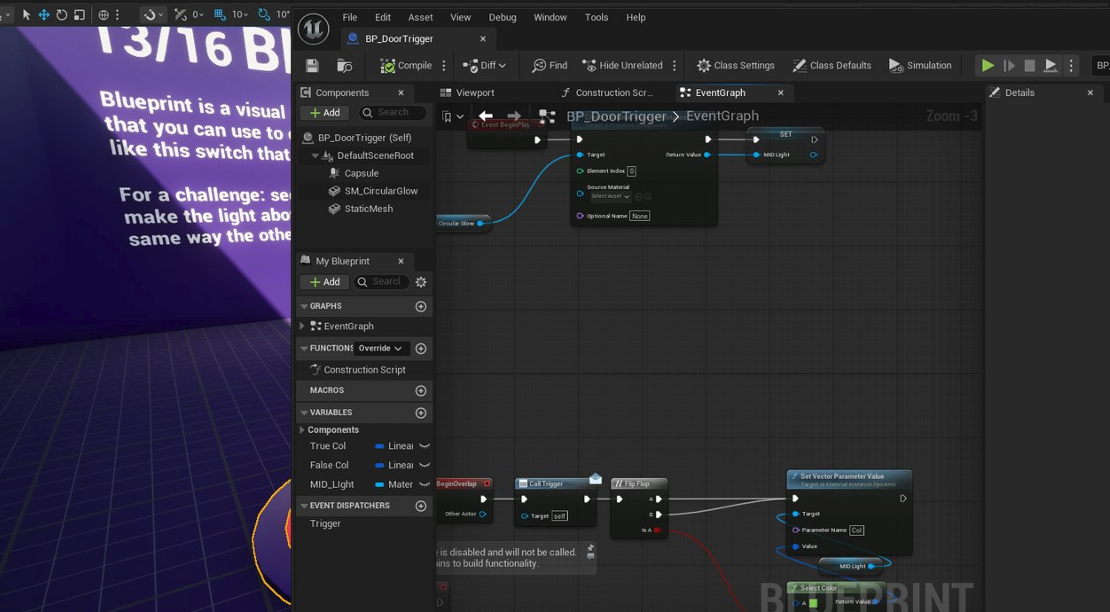
\includegraphics[width=0.9\textwidth]{images/ss-20-sequencer-flythrough.png}}
    \caption{Menu Add Objects pada Top Bar untuk menambahkan objek baru ke dalam level.}
    \label{fig:ss-addobject}
\end{figure}

    \item \textbf{Mengakses Content Drawer dengan CTRL+SPACE.} Saya membuka Content Drawer memakai shortcut \texttt{CTRL + SPACE}. Panel ini memuat aset project seperti mesh, material, dan texture, dan bisa dipakai untuk menarik aset langsung ke viewport.

    \item \textbf{Mengubah collision pada object.} Saya memilih objek \texttt{SM\_Ramp5} lalu membuka bagian Collision di panel Details. Dropdown Collision Presets menampilkan daftar preset seperti NoCollision, BlockAll, OverlapAll, BlockAllDynamic, Pawn, PhysicsActor, Trigger, sampai Ragdoll. Dari sini cara objek bereaksi terhadap tabrakan bisa diatur tanpa menyentuh mesh-nya.

\begin{figure}[H]
    \centering
    \customfbox{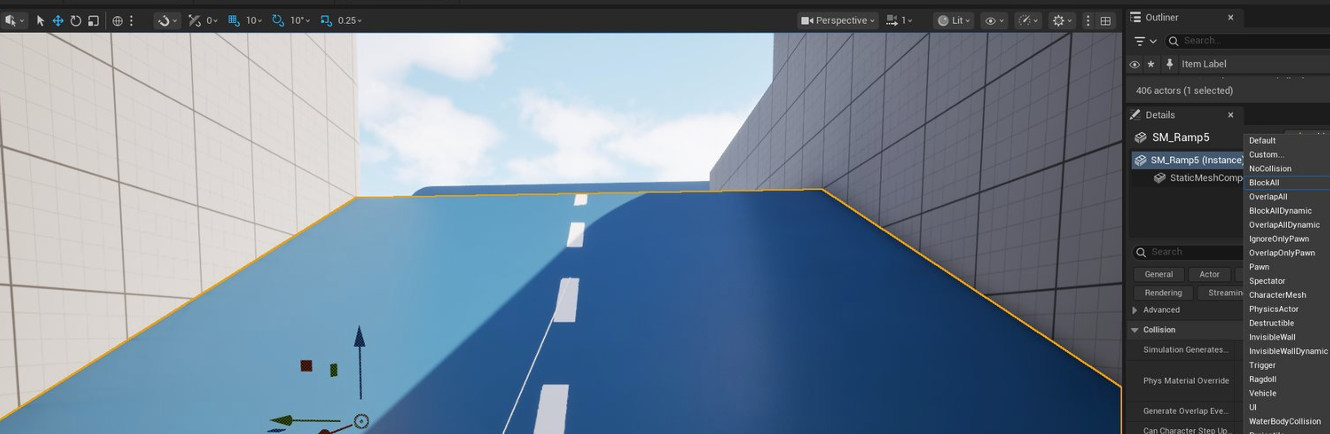
\includegraphics[width=0.9\textwidth]{images/ss-12-collision.png}}
    \caption{Dropdown Collision Presets pada Details milik SM\_Ramp5, dengan pilihan seperti BlockAll, OverlapAll, dan PhysicsActor.}
    \label{fig:ss-collision}
\end{figure}

    \item \textbf{Menghapus objek via Outliner.} Untuk objek yang posisinya sulit diklik langsung di Viewport, saya menyeleksinya dari daftar Outliner berdasarkan nama lalu menekan delete. Cara ini jauh lebih aman daripada menebak-nebak klik di scene yang objeknya bertumpuk.

    \item \textbf{Mengganti property material: Color, Metallic, Roughness.} Di stasiun 5/16 Materials, saya mengklik bola biru (\texttt{Sphere8}) dan membuka material \texttt{MI\_Intro\_Colorway} dari slot Element 0 di Details. Material editor terbuka dengan preview bola besar di kiri, dan Color Picker muncul saat Base Color diklik. Saya mengubah nilai RGB (R 0.025, G 0.014, B 0.104) untuk menggeser warna dasar, lalu mengamati efek nilai Metallic 0.0 dan Roughness 0.268 ke pantulan permukaannya.

\begin{figure}[H]
    \centering
    \customfbox{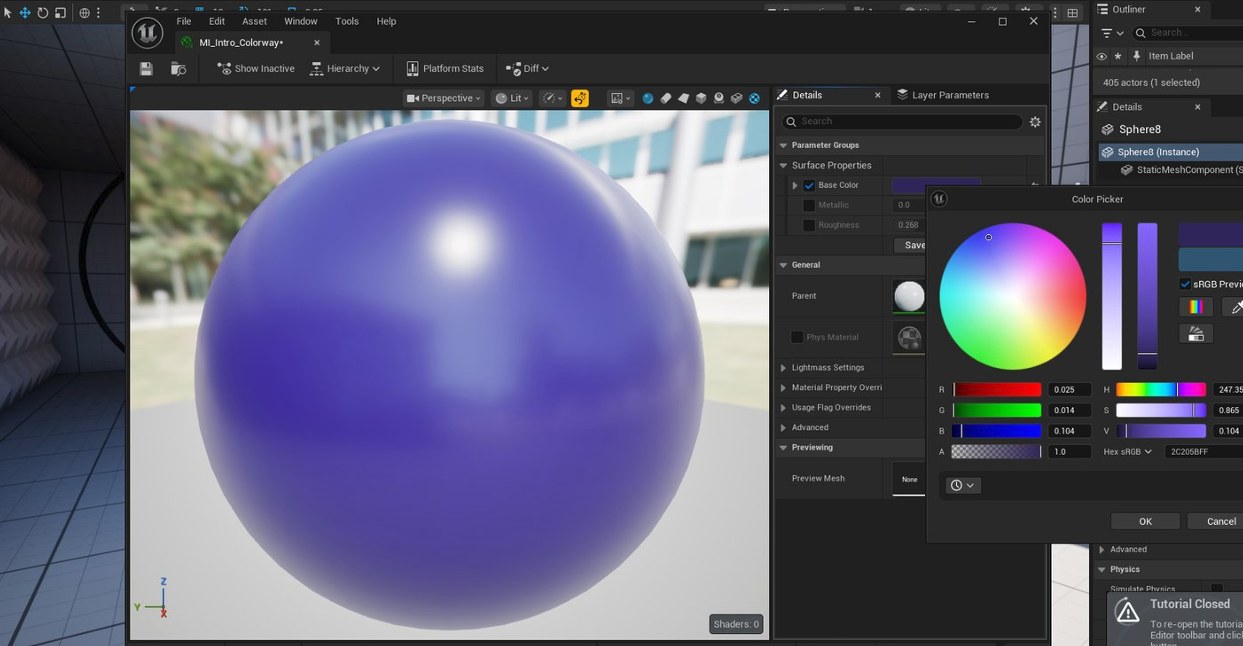
\includegraphics[width=0.9\textwidth]{images/ss-28-material-colorpicker.png}}
    \caption{Material editor MI\_Intro\_Colorway dengan Color Picker untuk mengubah Base Color, Metallic, dan Roughness.}
    \label{fig:ss-material-prop}
\end{figure}

    \item \textbf{Hot-swap material slot.} Masih di stasiun Materials, saya mencoba hot-swap dengan mengganti isi slot material Element 0 pada \texttt{Sphere8} langsung dari dropdown di Details. Material baru langsung terpasang ke bola tanpa perlu membuka editor material, jadi cara ini cocok untuk coba-coba tampilan dengan cepat.

\begin{figure}[H]
    \centering
    \customfbox{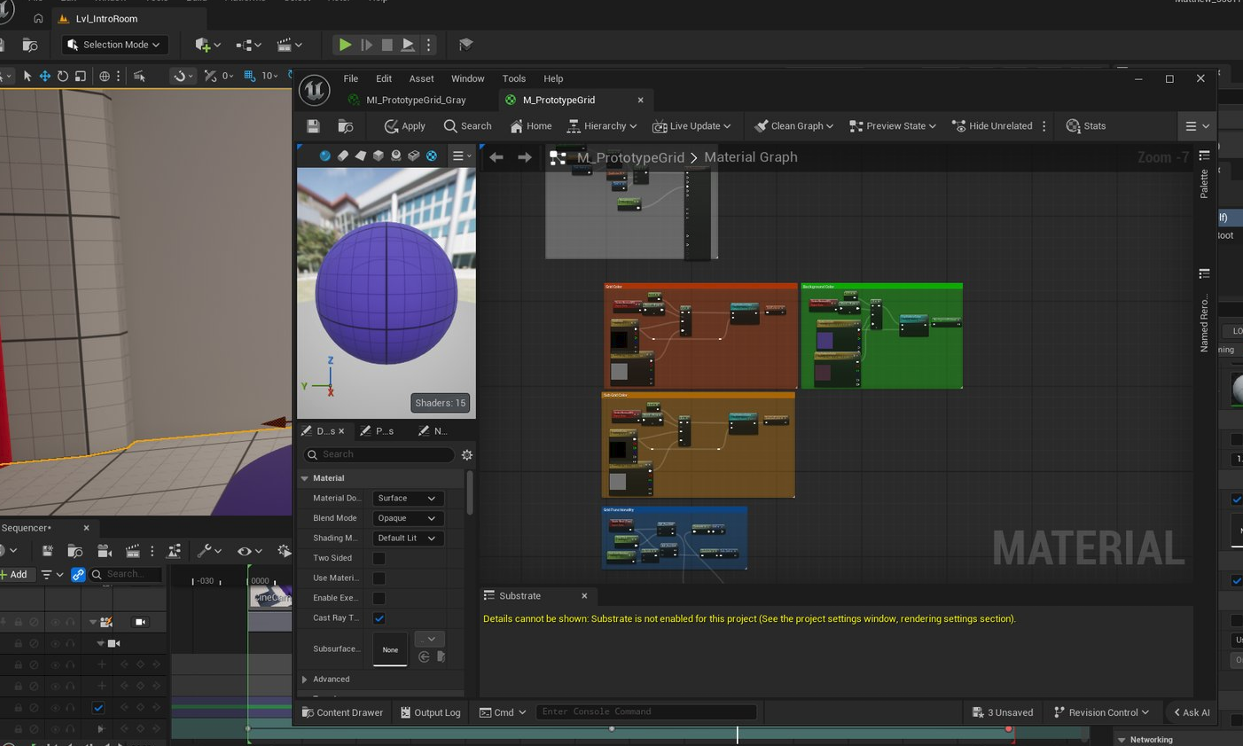
\includegraphics[width=0.9\textwidth]{images/ss-29-material-graph.png}}
    \caption{Hot-swap material pada slot Element 0 milik Sphere8 lewat dropdown di panel Details.}
    \label{fig:ss-hotswap}
\end{figure}
\end{enumerate}

\subsection{Pencahayaan, Fisika, Partikel, dan Logika}

\begin{enumerate}
    \item \textbf{Mengganti property particle system via Niagara Editor.} Saya membuka aset \texttt{NS\_DemoNiagara} dan Niagara Editor tampil dengan dua emitter: \texttt{OmnidirectionalBurst} dan \texttt{Ribbon\_Trail\_Leader}. Di panel Details saya mengubah Spawn Count pada modul Spawn Burst Instantaneous menjadi 170, dan perubahannya langsung kelihatan di preview. Editor ini juga menampilkan System Attributes dan timeline simulasi di bagian bawah.

\begin{figure}[H]
    \centering
    \customfbox{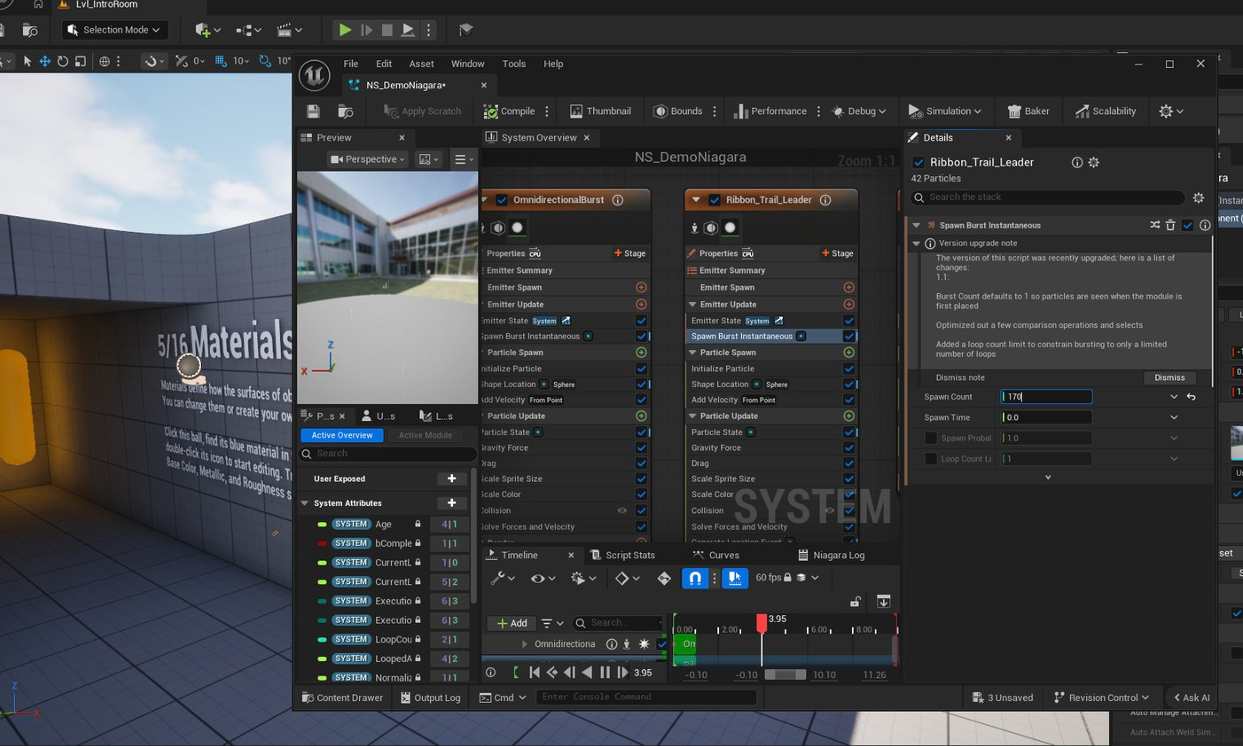
\includegraphics[width=0.9\textwidth]{images/ss-22-niagara.png}}
    \caption{Niagara Editor pada aset NS\_DemoNiagara dengan pengaturan Spawn Burst Instantaneous (Spawn Count 170).}
    \label{fig:ss-niagara}
\end{figure}

    \item \textbf{Mengganti property physics.} Di stasiun 9/16 Physics, saya memilih tumpukan kubus ungu \texttt{SM\_ChamferCube2} dan membuka kategori Physics di Details. Di sana saya mencentang Simulate Physics dengan Mass 5.0 kg, Linear Damping 0.01, dan Enable Gravity aktif. Saat di-play, kubus yang tadinya diam langsung jatuh dan saling menabrak mengikuti simulasi.

\begin{figure}[H]
    \centering
    \customfbox{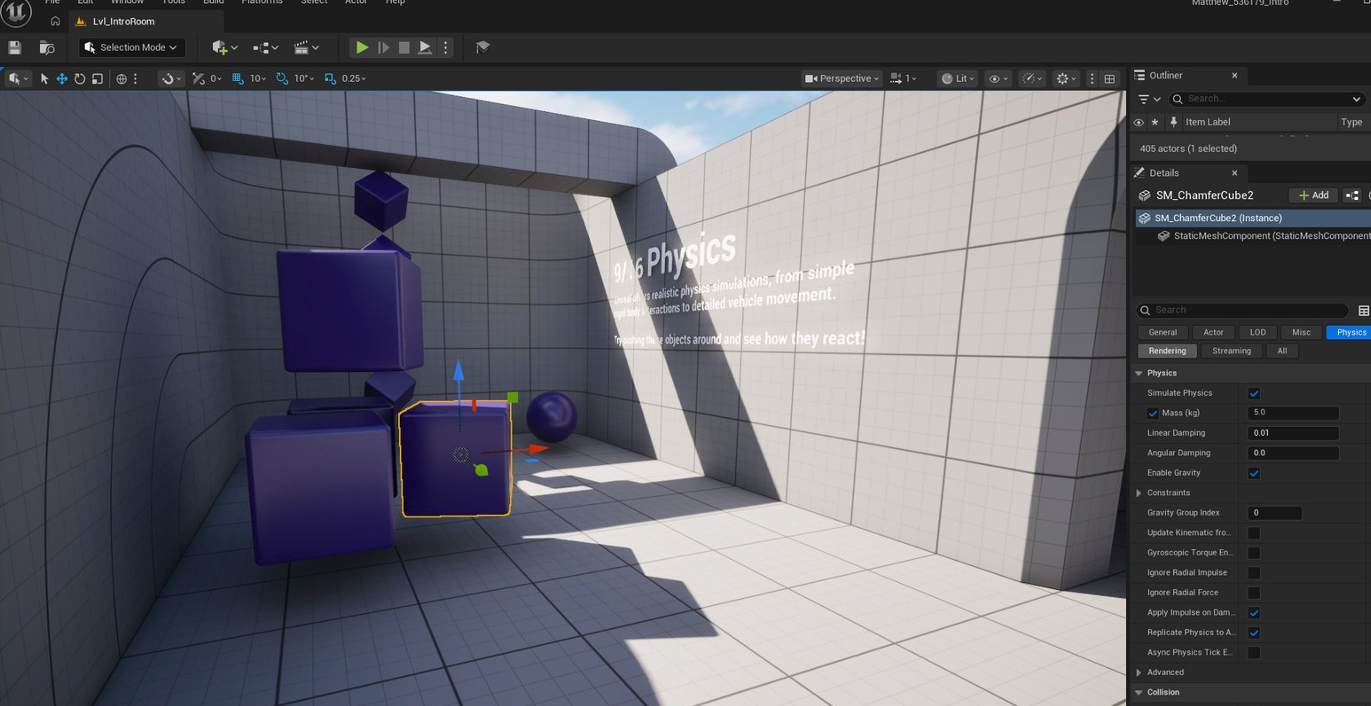
\includegraphics[width=0.9\textwidth]{images/ss-17-physics.png}}
    \caption{Pengaturan Physics pada SM\_ChamferCube2: Simulate Physics aktif dengan Mass 5.0 kg dan Enable Gravity.}
    \label{fig:ss-physics}
\end{figure}

    \item \textbf{Menambahkan Point Light dengan L + Left Click.} Di stasiun 8/16 Atmosphere, saya menambahkan Point Light dengan menahan tombol \texttt{L} lalu klik kiri di viewport. Cahaya langsung muncul di titik yang diklik. Saya juga memeriksa \texttt{DirectionalLight} di Outliner: intensitasnya 6.125057 lux dengan Temperature 6500, dan memutar rotasinya membuat langit berubah jadi nuansa senja oranye-ungu.

\begin{figure}[H]
    \centering
    \customfbox{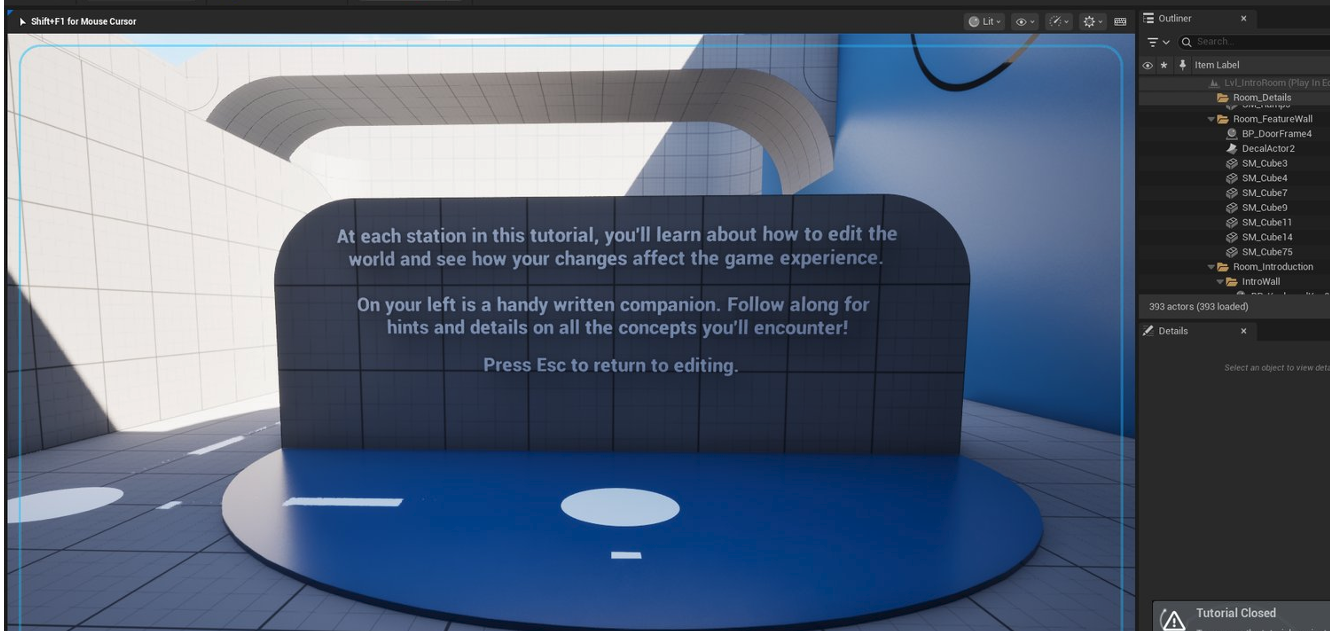
\includegraphics[width=0.9\textwidth]{images/ss-27-hasil-akhir.png}}
    \caption{Stasiun 8/16 Atmosphere dengan Point Light yang baru ditambahkan dan Details DirectionalLight (Intensity 6.125 lux, Temperature 6500).}
    \label{fig:ss-pointlight}
\end{figure}

    \item \textbf{Mencoba masuk ke sistem Sequencer.} Di stasiun 12/16 Sequencer, saya klik kanan objek sequence di Outliner lalu pilih Edit. Panel Sequencer terbuka di bawah viewport dengan timeline \texttt{NewLevelSequence} berisi track kamera \texttt{CineCameraActor}. Saat playhead digeser ke frame 269, viewport ikut menampilkan sudut kamera sinematik yang melintasi area stasiun 11/16 Animation dan 12/16 Sequencer.

\begin{figure}[H]
    \centering
    \customfbox{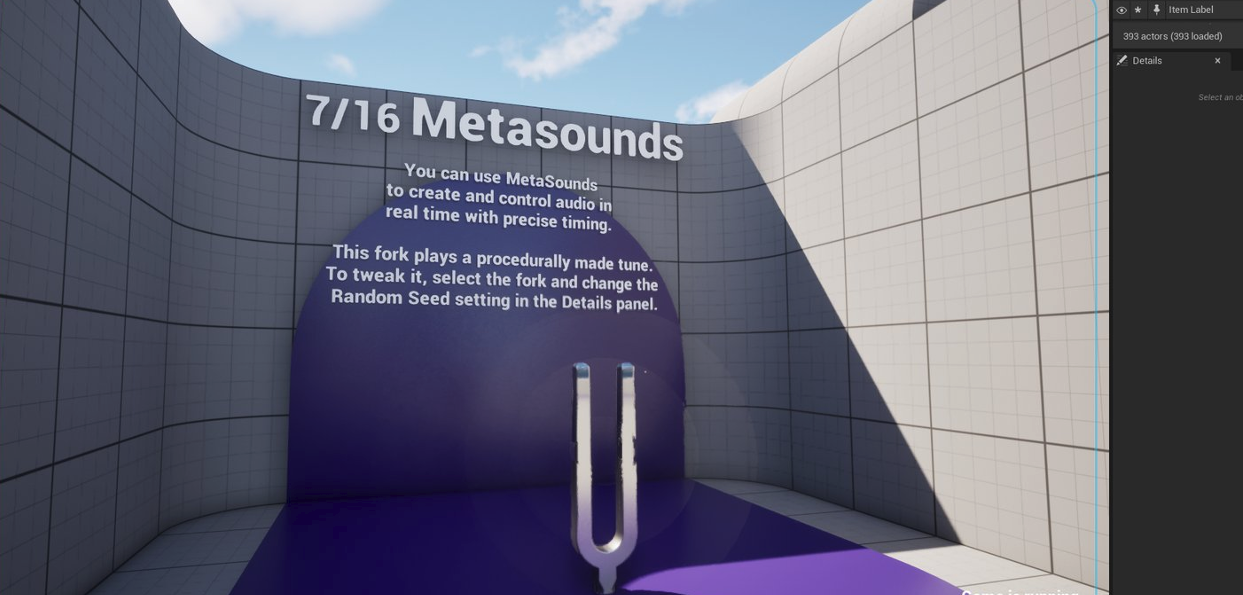
\includegraphics[width=0.9\textwidth]{images/ss-23-animation.png}}
    \caption{Editor Sequencer dengan timeline NewLevelSequence dan track CineCameraActor di stasiun 12/16.}
    \label{fig:ss-sequencer}
\end{figure}

    \item \textbf{Menjalankan camera flythrough.} Saat sequence dijalankan, kamera bergerak otomatis mengikuti track yang sudah dibuat. Viewport menampilkan label ``CineCameraActor'' dan flythrough melewati dinding-dinding stasiun dengan pencahayaan dramatis. Ada peringatan kecil ``Object Binding / Bound Object is missing!'' di timeline, tanda ada satu binding objek yang putus, tapi sequence tetap jalan.

\begin{figure}[H]
    \centering
    \customfbox{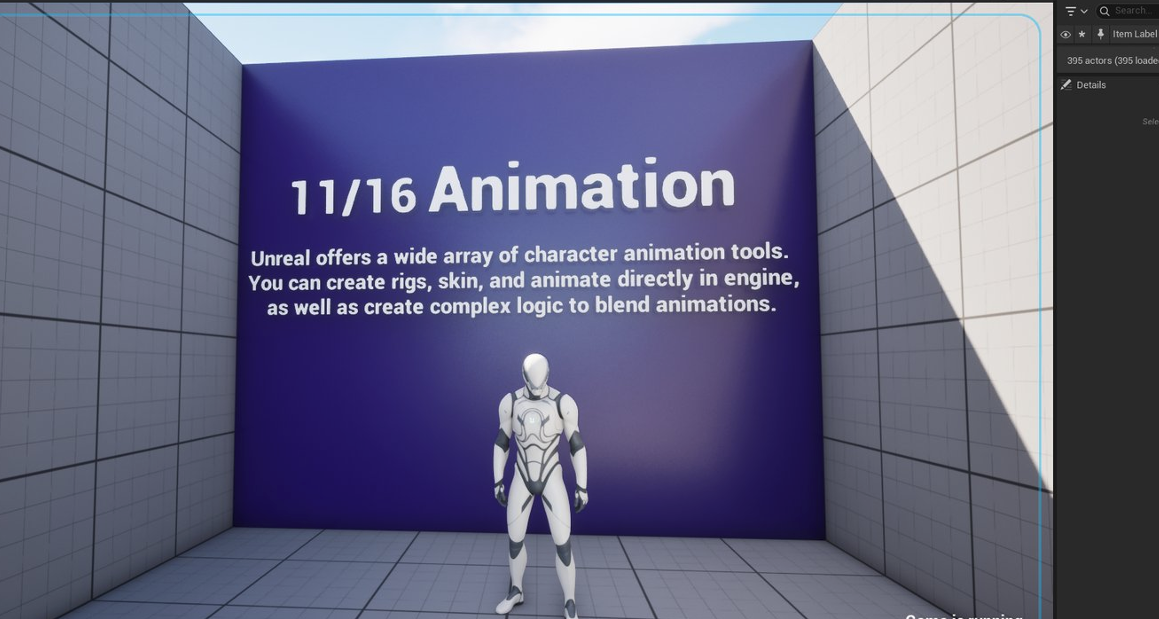
\includegraphics[width=0.9\textwidth]{images/ss-22-viewport-interior.png}}
    \caption{Camera flythrough Sequencer yang sedang berjalan melewati area stasiun dengan view CineCameraActor.}
    \label{fig:ss-flythrough}
\end{figure}

    \item \textbf{Mengganti logic object via Blueprint.} Di stasiun 13/16 Blueprint, saya membuka \texttt{BP\_DoorTrigger}. EventGraph-nya berisi rangkaian node: BeginOverlap memicu Call Trigger, masuk ke Flip Flop, lalu bercabang ke Set Vector Parameter Value untuk mengganti warna material \texttt{MID\_Light}. Di panel Components terlihat variabel True Col, False Col, dan MID\_Light. Dari sini kelihatan bagaimana logika visual menggantikan kode untuk mengatur perilaku switch dan lampu.

\begin{figure}[H]
    \centering
    \customfbox{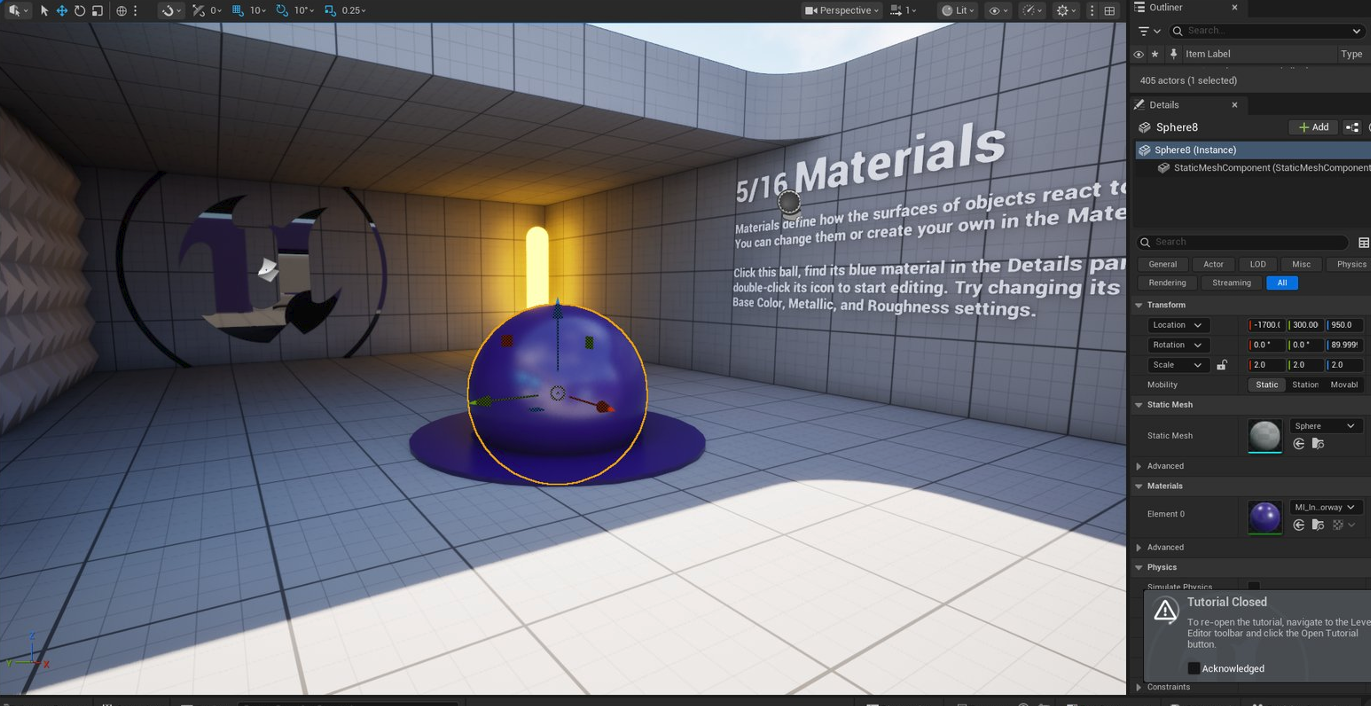
\includegraphics[width=0.9\textwidth]{images/ss-21-blueprint.png}}
    \caption{EventGraph Blueprint BP\_DoorTrigger dengan node BeginOverlap, Flip Flop, dan Set Vector Parameter Value.}
    \label{fig:ss-blueprint}
\end{figure}

    \item \textbf{Save project dengan CTRL+S.} Setelah semua percobaan selesai, saya menyimpan perubahan level dengan tombol Save di Top Bar dan memastikannya lewat shortcut \texttt{CTRL+S}.
\end{enumerate}

\section{Hasil Akhir}
Di akhir praktikum, project \texttt{HAFIDZ\_535493\_Intro} berhasil dibuat dari template Intro To Unreal di Unreal Engine 5.8.1 dan seluruh alur navigasi editor sudah saya coba langsung. Levelnya sudah berisi objek dengan material yang diganti lewat Color Picker maupun hot-swap slot, collision dan physics yang diatur dari Details, Point Light tambahan di area Atmosphere, particle Niagara yang Spawn Count-nya dimodifikasi, serta sequence kamera yang berjalan lewat Sequencer. Terakhir, semuanya saya simpan dengan aman.

\begin{figure}[H]
    \centering
    \customfbox{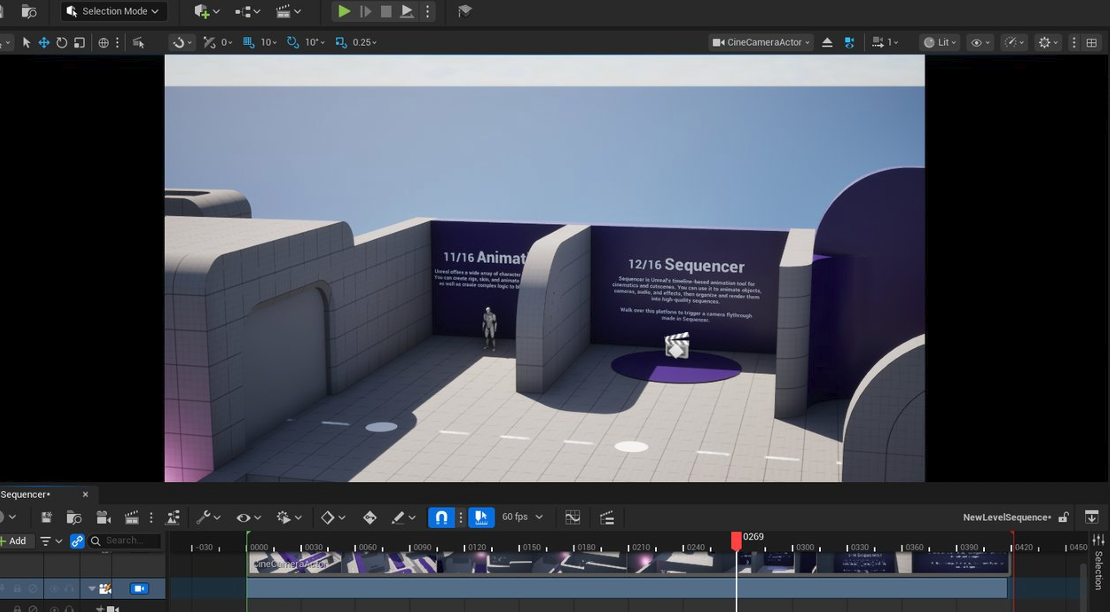
\includegraphics[width=0.9\textwidth]{images/ss-16-metasounds.png}}
    \caption{Hasil akhir penjelajahan Lvl\_IntroRoom sampai stasiun 7/16 Metasounds setelah seluruh rangkaian modifikasi objek, material, cahaya, dan physics selesai dikerjakan.}
    \label{fig:hasil-akhir}
\end{figure}

Hasil ini menunjukkan saya bisa mengikuti instruksi modul dari awal Epic Games Launcher sampai manipulasi editor dan komponen visual, sesuai ketentuan Format Tugas Modul 2 \cite{modul2}.

\clearpage

\chapter{Kesimpulan}
Dari praktikum Pertemuan 2 Navigate Unreal Engine 5.8, saya simpulkan bahwa Unreal Engine 5.8 adalah engine real-time lintas platform buatan Epic Games yang gratis dipakai sampai batas royalti komersial 1 juta USD. Lewat Epic Games Launcher saya bisa mengelola instalasi engine dan project, termasuk antisipasi warning file \texttt{.uproject}. Antarmuka editor yang terdiri dari Outliner, Details, Viewport, Content Drawer, dan Top Bar ternyata memberikan workflow yang terpusat dan enak dipakai untuk menata level.

Saya juga jadi paham cara melakukan transformasi objek (Move/Rotate/Scale), mengatur grid, menambah dan menghapus objek via Outliner, mengganti material baik lewat Color Picker maupun hot-swap slot, serta mengatur collision dan physics dari Details. Penambahan Point Light dengan \texttt{L + Left Click} dan pengaturan particle via Niagara Editor menambah wawasan soal aspek visual. Akses ke Sequencer dan Blueprint memberi gambaran awal tentang cinematics dan visual scripting, dan semuanya saya tutup dengan menyimpan project lewat \texttt{CTRL+S}. Seluruh rangkaian ini sesuai tujuan praktikum dan jadi bekal untuk materi pengembangan game di pertemuan berikutnya.

\clearpage
\addcontentsline{toc}{chapter}{Daftar Pustaka}
\renewcommand{\bibname}{Daftar Pustaka}
\begin{thebibliography}{99}
    \bibitem{modul2} Modul Praktikum Pengembangan Game Pertemuan 2 --- Navigate Unreal Engine 5.8, T.A. 2026/2027. Semester Gasal, Universitas Gadjah Mada.
    \bibitem{epic-unreal} Epic Games, ``Unreal Engine 5 Documentation'', 2026. [Online]. Tersedia: \url{https://dev.epicgames.com/documentation/unreal-engine/}.
    \bibitem{epic-variants} Epic Games, ``Variants in Game Templates'', 2026. [Online]. Tersedia: \url{https://dev.epicgames.com/documentation/unreal-engine/variants-in-game-templates}.
    \bibitem{kurogames} Kuro Games, ``Company Introduction'', 2026. [Online]. Tersedia: \url{https://www.kurogames.com/introduction}.
    \bibitem{wuthering-cover} PCGamingWiki, ``Wuthering Waves Cover'', 2026. [Online]. Tersedia: \url{https://images.pcgamingwiki.com/4/47/Wuthering_Waves_cover.jpg}.
    \bibitem{epic-naming} Epic Games, ``Recommended Asset Naming Conventions in Unreal Engine Projects'', 2026. [Online]. Tersedia: \url{https://dev.epicgames.com/documentation/en-us/unreal-engine/recommended-asset-naming-conventions-in-unreal-engine-projects}.
\end{thebibliography}

\end{document}
